%
% ff.tex -- Kryptographie und endliche Körper
%
% (c) 2020 Prof Dr Andreas Müller, Hochschule Rapperswil
%

\section{Kryptographie und endliche Körper
\label{buch:section:kryptographie-und-endliche-koerper}}
\rhead{Kryptographie und endliche Körper}

\subsection{Potenzen in $\mathbb{F}_p$ und diskreter Logarithmus
\label{buch:subsection:potenzen-diskreter-logarithmus}}
Für kryptographische Anwendungen wird eine einfach zu berechnende
Funktion benötigt,
die ohne zusätzliches Wissen, üblicherweise der Schlüssel genannt,
nicht ohne weiteres umkehrbar ist.
Die arithmetischen Operationen in einem endlichen Körper sind
mit geringem Aufwand durchführbar.
Für die ``schwierigste'' Operation, die Division, steht der
euklidische Algorithmus zur Verfügung.

Die nächstschwierigere Operation ist die Potenzfunktion.
Für $g\in \Bbbk$ und $a\in\mathbb{N}$ ist die Potenz $g^a\in\Bbbk$
natürlich durch die wiederholte Multiplikation definiert.
In der Praxis werden aber $g$ und $a$ Zahlen mit vielen Binärstellen
sein, die die wiederholte Multiplikation ist daher sicher nicht
effizient, das Kriterium der einfachen Berechenbarkeit scheint
also nicht erfüllt.
Der folgende Algorithmus berechnet die Potenz in $O(\log_2 a)$
Multiplikationen.

\begin{algorithmus}[Divide-and-conquer]
\label{buch:crypto:algo:divide-and-conquer}
Sei $a=a_0 + a_12^1 + a_22^2 + \dots + a_k2^k$ die Binärdarstellung
der Zahl $a$.
\begin{enumerate}
\item setze $f=g$, $x=1$, $i=0$
\label{divide-and-conquer-1}
\item solange $i\ge k$ ist, führe aus
\label{divide-and-conquer-2}
\begin{enumerate}
\item
\label{divide-and-conquer-3}
falls $a_i=1$ setze $x \coloneqq x \cdot f$
\item
\label{divide-and-conquer-4}
$i \coloneqq i+1$ und $f\coloneqq f\cdot f$
\end{enumerate}
\end{enumerate}
Die Potenz $x=g^a$ kann so in $O(\log_2a)$ Multiplikationen
berechnet werden.
\end{algorithmus}

\begin{proof}[Beweis]
Die Initalisierung in Schritt~\ref{divide-and-conquer-1} stellt sicher,
dass $x$ den Wert $g^0$ hat. 
Schritt~\ref{divide-and-conquer-4} stellt sicher,
dass die Variable $f$ immer den Wert $g^{2^i}$ hat.
Im Schritt~\ref{divide-and-conquer-3} wird zu $x$ die Potenz
$g^{a_i2^i}$ hinzumultipliziert.
Am Ende des Algorithmus hat daher $x$ den Wert
\[
x = g^{a_02^0} \cdot g^{a_12^1} \cdot g^{a_22^2} \cdot\ldots\cdot 2^{a_k2^k}
=
g^{a_0+a_12+a_22^2+\dots+a_k2^k}
=
g^a.
\]
Die Schleife wird $\lfloor1+\log_2ab\rfloor$ mal durchlaufen.
In jedem Fall wird auf jeden Fall die Multiplikation in 
Schritt~\ref{divide-and-conquer-4} durchgeführt
und im schlimmsten Fall auch noch die Multiplikation in
Schritt~\ref{divide-and-conquer-3}.
Es werden also nicht mehr als $2\lfloor 1+\log_2a\rfloor=O(\log_2a)$
Multiplikationen durchgeführt.
\end{proof}

\begin{beispiel}
Man berechne die Potenz $7^{2021}$ in $\mathbb{F}_p$.
Die Binärdarstellung von 2021 ist $2021_{10}=\texttt{11111100101}_2$.
Wir stellen die nötigen Operationen des
Algorithmus~\ref{buch:crypto:algo:divide-and-conquer} in der folgenden
Tabelle
\begin{center}
\begin{tabular}{|>{$}r<{$}|>{$}r<{$}|>{$}r<{$}|>{$}r<{$}|}
\hline
 i&   f& a_i&    x\\
\hline
 0&   7&   1&    7\\
 1&  49&   0&    7\\
 2&1110&   1&   24\\
 3& 486&   0&   24\\
 4&1234&   0&   24\\
 5& 667&   1&  516\\
 6& 785&   1&  977\\
 7& 418&   1&  430\\
 8& 439&   1&  284\\
 9& 362&   1&  819\\
10& 653&   1&  333\\
\hline
\end{tabular}
\end{center}
Daraus liest man ab, dass $7^{2021}=333\in\mathbb{F}_{1291}$.
\end{beispiel}

Die Tabelle suggeriert, dass die Potenzen von $g$ ``wild'', also
scheinbar ohne System in $\mathbb{F}_p$ herumspringen.
Dies deutet an, dass die Umkehrung der Exponentialfunktion in $\mathbb{F}_p$
schwierig ist.
Die Umkehrfunktion der Exponentialfunktion, die Umkehrfunktion von 
$x\mapsto g^x$ in $\mathbb{F}_p$ heisst der {\em diskrete Logarithmus}.
\index{diskreter Logarithmus}%
Tatsächlich ist der diskrete Logarithmus ähnlich schwierig zu bestimmen
wie das Faktorisieren von Zahlen, die das Produkt grosser
Primafaktoren ähnlicher Grössenordnung wie $p$ sind.
Die Funktion $x\mapsto g^x$ ist die gesuchte, schwierig zu invertierende
Funktion.

Auf dern ersten Blick scheint der
Algorithmus~\ref{buch:crypto:algo:divide-and-conquer}
den Nachteil zu haben, dass erst die Binärdarstellung der Zahl $a$ 
ermittelt werden muss.
In einem Computer ist dies aber normalerweise kein Problem, da $a$
im Computer ohnehin binär dargestellt ist.
Die Binärziffern werden in der Reihenfolge vom niederwertigsten zum
höchstwertigen Bit benötigt.
Die folgende Modifikation des Algorithmus ermittelt laufend
auch die Binärstellen von $a$.
Die dazu notwendigen Operationen sind im Binärsystem besonders
effizient implementierbar, die Division durch 2 ist ein Bitshift, der
Rest ist einfach das niederwertigste Bit der Zahl.

\begin{algorithmus}
\label{buch:crypto:algo:divide-and-conquer2}
\begin{enumerate}
\item
Setze $f=g$, $x=1$, $i=0$
\item
Solange $a>0$ ist, führe aus
\begin{enumerate}
\item
Verwende den euklidischen Algorithmus um $r$ und $b$ zu bestimmen mit $a=2b+r$
\item
Falls $r=1$ setze $x \coloneqq x \cdot f$
\item
$i \coloneqq i+1$, $a = b$ und $f\coloneqq f\cdot f$
\end{enumerate}
\end{enumerate}
Die Potenz $x=g^a$ kann so in $O(\log_2a)$ Multiplikationen
berechnet werden.
\end{algorithmus}


%
% Diffie-Hellman Schlüsseltausch
%
\subsection{Diffie-Hellman-Schlüsseltausch
\label{buch:subsection:diffie-hellman}}
Eine Grundaufgabe der Verschlüsselung im Internet ist, dass zwei
Kommunikationspartner einen gemeinsamen Schlüssel für die Verschlüsselung
der Daten aushandeln können müssen.
Es muss davon ausgegangen werden, dass die Kommunikation abgehört wird.
Trotzdem soll es für einen Lauscher nicht möglich sein, den 
ausgehandelten Schlüssel zu ermitteln.

% XXX Historisches zu Diffie und Hellman

Die beiden Partner $A$ und $B$ einigen sich zunächst auf eine Zahl $g$,
die öffentlich bekannt sein darf.
Weiter erzeugen sie eine zufällige Zahl $a$ und $b$, die sie geheim
halten.
Das Verfahren soll aus diesen beiden Zahlen einen Schlüssel erzeugen,
den beide Partner berechnen können, ohne dass sie $a$ oder $b$ 
übermitteln müssen.
Die beiden Zahlen werden daher auch die privaten Schlüssel genannt.

Die Idee von Diffie und Hellman ist jetzt, die Werte $x=g^a$ und $y=g^b$
zu übertragen.
In $\mathbb{R}$ würden dadurch natürlich dem Lauscher auch $a$ offenbart,
er könnte einfach $a=\log_g x$ berechnen.
Ebenso kann auch $b$ als $b=\log_g y$ erhalten werden, die beiden
privaten Schlüssel wären also nicht mehr privat.
Statt der Potenzfunktion in $\mathbb{R}$ muss also eine Funktion
verwendet werden, die nicht so leicht umgekehrt werden kann.
Die Potenzfunktion in $\mathbb{F}_p$ erfüllt genau diese Eigenschaft.
Die Kommunikationspartner einigen sich also auch noch auf die (grosse)
Primzahl $p$ und übermitteln $x=g^a\in\mathbb{F}_p$ und
$y=g^b\in\mathbb{F}_p$.

\begin{figure}
\centering
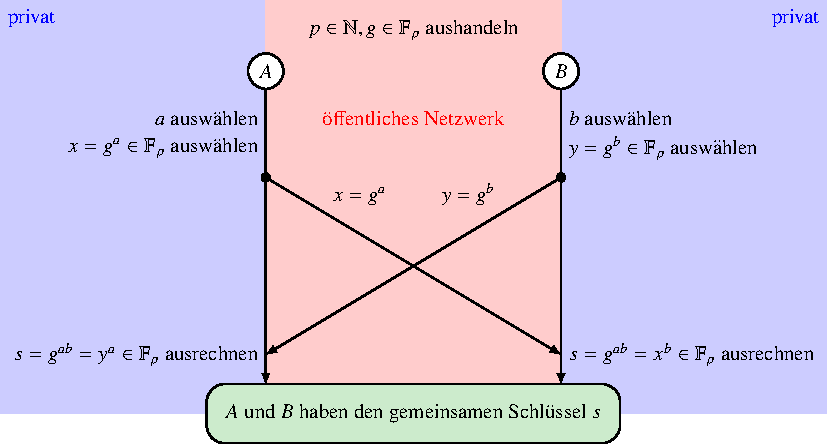
\includegraphics{chapters/90-crypto/images/dh.pdf}
\caption{Schlüsselaustausch nach Diffie-Hellman.
Die Kommunikationspartner $A$ und $B$ einigen sich öffentlich auf
$p\in\mathbb{N}$ und $g\in\mathbb{F}_p$.
$A$ wählt dann einen privaten Schlüssel $a\in\mathbb{N}$ und
$B$ wählt $b\in\mathbb{N}$, sie tauschen dann $x=g^a$ und $y=g^b$
aus.
$A$ erhält den gemeinsamen Schlüssel aus $y^a$, $B$ erhält ihn
aus $x^b$.
\label{buch:crypto:fig:dh}}
\end{figure}

Aus $x$ und $y$ muss jetzt der gemeinsame Schlüssel abgeleitet werden.
$A$ kennt $y=g^b$ und $a$, $B$ kennt $x=g^a$ und $b$.
Beide können die Zahl $s=g^{ab}\in\mathbb{F}_p$ berechnen.
$A$ macht das, indem er $y^a=(g^b)^a = g^{ab}$ rechnet,
$B$ rechnet $x^b = (g^a)^b = g^{ab}$, beide natürlich in $\mathbb{F}_p$.
Der Lauscher kann aber $g^{ab}$ nicht ermitteln, dazu müsste er
$a$ oder $b$ ermitteln können.
Die Zahl $s=g^{ab}$ kann also als gemeinsamer Schlüssel verwendet
werden.



\subsection{Elliptische Kurven
\label{buch:subsection:elliptische-kurven}}
Das Diffie-Hellman-Verfahren basiert auf der Schwierigkeit, in einem 
Körper $\mathbb{F}_p$ die Gleichung $a^x=b$ nach $x$ aufzulösen.
Die Addition in $\mathbb{F}_p$ wird dazu nicht benötigt.
Es reicht, eine Menge mit einer Multiplikation zu haben, in der das
die Gleichung $a^x=b$ schwierig zu lösen ist.
Ein Gruppe wäre also durchaus ausreichend.

Ein Kandidat für eine solche Gruppe könnte der Einheitskreis
$S^1=\{z\in\mathbb{C}\;|\; |z|=1\}$ in der komplexen Ebene sein.
Wählt man eine Zahl $g=e^{i\alpha}$, wobei $\alpha$ ein irrationales
Vielfaches von $\pi$ ist, dann sind alle Potenzen $g^n$ für natürliche
Exponenten voneinander verschieden.
Wäre nämlich $g^{n_1}=g^{n_2}$, dann wäre $e^{i\alpha(n_1-n_2)}=1$ und
somit müsste $\alpha=2k\pi/(n_1-n_2)$ sein.
Damit wäre aber $\alpha$ ein rationales Vielfaches von $\pi$, im Widerspruch
zur Voraussetzung.
Die Abbildung $n\mapsto g^n\in S^1$ ist auf den ersten Blick etwa ähnlich
undurchschaubar wie die Abbildung $n\mapsto g^n\in\mathbb{F}_p$.
Es gibt zwar die komplexe Logarithmusfunktion, mit der man $n$ bestimmen
kann, dazu muss man aber den Wert von $g^n$ mit beliebiger Genauigkeit
kennen, denn die Werte von $g^n$ können beliebig nahe beieinander liegen.

Der Einheitskreis ist die Lösungsmenge der Gleichung $x^2+y^2=1$ für
reelle Koordinaten $x$ und $y$,
doch Rundungsunsicherheiten verunmöglichen den Einsatz in einem 
Verfahren ähnlich dem Diffie-Hellman-Verfahren.
Dieses Problem kann gelöst werden, indem für die Variablen Werte
aus einem endlichen Körper verwendet werden.
Gesucht ist also eine Gleichung in zwei Variablen, deren Lösungsmenge
in einem endlichen Körper eine Gruppenstruktur trägt.
Die Lösungsmenge ist eine ``Kurve'' von Punkten mit
Koordinaten in einem endlichen Körper.

In diesem Abschnitt wird gezeigt, dass sogenannte elliptische Kurven
über endlichen Körpern genau die verlangen Eigenschaften haben.

\subsubsection{Elliptische Kurven}
Elliptische Kurven sind Lösungen einer Gleichung der Form
\begin{equation}
Y^2+XY=X^3+aX+b
\label{buch:crypto:eqn:ellipticcurve}
\end{equation}
mit Werten von $X$ und $Y$ in einem geeigneten Körper.
Die Koeffizienten $a$ und $b$ müssen so gewählt werden, dass die
Gleichung~\eqref{buch:crypto:eqn:ellipticcurve} genügend viele
Lösungen hat.
Über den komplexen Zahlen hat die Gleichung natürlich für jede Wahl von
$X$ drei Lösungen.
Für einen endlichen Körper können wir dies im allgemeinen nicht erwarten,
aber wenn wir genügend viele Wurzeln zu $\mathbb{F}$ hinzufügen können wir
mindestens erreichen, dass die Lösungsmenge so viele Elemente hat, 
dass ein Versuch, die Gleichung $g^x=b$ mittels Durchprobierens zu
lösen, zum Scheitern verurteil ist.

\begin{definition}
\label{buch:crypto:def:ellipticcurve}
Die {\em elliptische Kurve} $E_{a,b}(\Bbbk)$ über dem Körper $\Bbbk$ ist 
die Menge
\[
E_{a,b}(\Bbbk)
=
\{(X,Y)\in\Bbbk^2\;|\;Y^2+XY=X^3+aX+b\},
\]
für $a,b\in\Bbbk$.
\end{definition}

Um die Anschauung zu vereinfachen, werden wir elliptische Kurven über
dem Körper $\mathbb{R}$ visualisieren.
Die daraus gewonnenen geometrischen Einsichten werden wir anschliessend
algebraisch umsetzen.
In den reellen Zahlen kann man die
Gleichung~\eqref{buch:crypto:eqn:ellipticcurve}
noch etwas vereinfachen.
Indem man in \eqref{buch:crypto:eqn:ellipticcurve} 
quadratisch ergänzt, bekommt man
\begin{align}
Y^2 + XY + \frac14X^2 &= X^3+\frac14 X^2 +aX+b
\notag
\\
\Rightarrow\qquad
v^2&=X^3+\frac14X^2+aX+b,
\label{buch:crypto:eqn:ell2}
\end{align}
indem man $v=Y+\frac12X$ setzt.
Man beachte, dass man diese Substition nur machen kann, wenn $\frac12$
definiert ist.
In $\mathbb{R}$ ist dies kein Problem, aber genau über den Körpern
mit Charakteristik $2$, die wir für die Computer-Implementation
bevorzugen, ist dies nicht möglich.
Es geht hier aber nur um die Visualisierung.

Auch die Form \eqref{buch:crypto:eqn:ell2} lässt sich noch etwas 
vereinfachen.
Setzt man $X=u-\frac1{12}$, dann verschwindet nach einiger Rechnung,
die wir hier nicht durchführen wollen, der quadratische Term
auf der rechten Seite.
Die interessierenden Punkte sind Lösungen der einfacheren Gleichung
\begin{equation}
v^2
=
u^3+\biggl(a-\frac{1}{48}\biggr)u + b-\frac{a}{12}+\frac{1}{864}
=
u^3+Au+B.
\label{buch:crypto:ellvereinfacht}
\end{equation}
In dieser Form ist mit $(u,v)$ immer auch $(u,-v)$ eine Lösung,
die Kurve ist symmetrisch bezüglich der $u$-Achse.
Ebenso kann man ablesen, dass nur diejenigen $u$-Werte möglich sind,
für die das kubische Polynom $u^3+Au+B$ auf der rechten Seite von
\eqref{buch:crypto:ellvereinfacht}
nicht negativ ist.

Sind $u_1$, $u_2$ und $u_3$ die Nullstellen des kubischen Polynoms
auf der rechten Seite von~\eqref{buch:crypto:ellvereinfacht}, folgt
\[
v^2
=
(u-u_1)(u-u_2)(u-u_3)
=
u^3
-(u_1+u_2+u_3)u^2
+(u_1u_2+u_1u_3+u_2u_3)u
-
u_1u_2u_3.
\]
Durch Koeffizientenvergleich sieht man, dass $u_1+u_2+u_3=0$ sein muss.
\begin{figure}
\centering
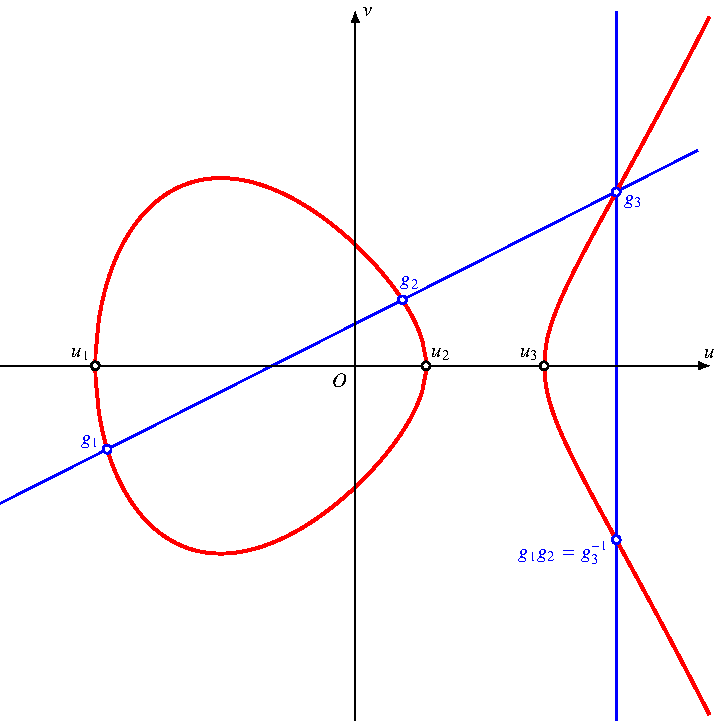
\includegraphics{chapters/90-crypto/images/elliptic.pdf}
\caption{Elliptische Kurve in $\mathbb{R}$ in der Form
$v^2=u^3+Au+B$ mit Nullstellen $u_1$, $u_2$ und $u_3$ des
kubischen Polynoms auf der rechten Seite.
Die blauen Punkte und Geraden illustrieren die Definition der
Gruppenoperation in der elliptischen Kurve.
\label{buch:crypto:fig:elliptischekurve}}
\end{figure}
Abbildung~\ref{buch:crypto:fig:elliptischekurve}
zeigt eine elliptische Kurve in der Ebene.

\subsubsection{Geometrische Definition der Gruppenoperation}
In der speziellen Form \ref{buch:crypto:ellvereinfacht} ist die
elliptische Kurve symmetrisch unter Spiegelung an der $u$-Achse.
Die Spiegelung ist eine Involution, zweimalige Ausführung führt auf
den ursprünglichen Punkt zurück.
Die Inverse in einer Gruppe hat diese Eigenschaft auch, es ist
daher naheliegend, den gespiegelten Punkt als die Inverse eines
Elementes zu nehmen.

Eine Gerade durch zwei Punkte der
in Abbildung~\ref{buch:crypto:fig:elliptischekurve}
dargestellten Kurve schneidet die Kurve ein drittes Mal.
Die Gruppenoperation wird so definiert, dass drei Punkte der Kurve
auf einer Geraden das Gruppenprodukt $e$ haben.
Da aus $g_1g_2g_3=e$ folgt $g_3=(g_1g_2)^{-1}$ oder
$g_1g_2=g_3^{-1}$, erhält man das Gruppenprodukt zweier Elemente
auf der elliptischen Kurve indem erst den dritten Schnittpunkt
ermittelt und diesen dann an der $u$-Achse spiegelt.

Die geometrische Konstruktion schlägt fehl, wenn $g_1=g_2$ ist.
In diesem Fall kann man die Tangente im Punkt $g_1$ an die Kurve 
verwenden.
Dieser Fall tritt zum Beispiel auch in den drei Punkten 
$(u_1,0)$, $(u_2,0)$ und $(u_3,0)$ ein.

Um das neutrale Element der Gruppe zu finden, können wir 
zwei Punkte $g$ und $g^{-1}$ miteinander verknüpfen.
Die Gerade durch $g$ und $g^{-1}$ schneidet aber die Kurve
kein drittes Mal.
Ausserdem sind alle Geraden durch $g$ und $g^{-1}$ für verschiedene
$g$ parallel.
Das neutrale Element entspricht also einem unendlich weit entfernten Punkt.
Das neutrale Element entsteht immer dann als Produkt, wenn zwei
Punkte die gleiche $u$-Koordinaten haben.

\subsubsection{Gruppenoperation, algebraische Konstruktion}
Nach den geometrischen Vorarbeiten zur Definition der Gruppenoperation
kann können wir die Konstruktion jetzt algebraisch umsetzen.

Zunächst überlegen wir uns wieder eine Involution, welche als Inverse
dienen kann.
Dazu beachten wir, dass die linke Seite der definierenden Gleichung
\begin{equation}
Y^2+XY=X^3-aX+b.
\label{buch:crypto:eqn:grupopgl}
\end{equation}
auch als $Y(Y+X)$ geschrieben werden kann.
Die Abbildung $Y\mapsto -X-Y$ macht daraus
\[
(-X-Y)(-X-Y+X)=(X+Y)Y,
\]
dies ist also die gesuchte Involution.

Seien also $g_1=(x_1,y_1)$ und $g_2=(x_2,y_2)$ zwei verschiedene Lösungen
der Gleichung \eqref{buch:crypto:eqn:grupopgl}
Als erstes brauchen wir eine Gleichung für die Gerade durch die beiden
Punkte.
Sei also $l(X,Y)$ eine Linearform derart, dass $l(g_1)=d$ und $l(g_2)=d$
für ein geeignetes $d\in\Bbbk$.
Dann gilt auch für die Punkte
\[
g(t) = tg_1 + (1-t)g_2
\qquad\Rightarrow\qquad
l(g(t))
=
tl(g_1) + (1-t)l(g_2)
=
tc+(1-t)c
=
(t+1-t)c
=c,
\]
jeder Punkt der Geraden durch $g_1$ und $g_2$ lässt sich in dieser Form
schreiben.

Setzt man jetzt $g(t)$ in die Gleichung ein, erhält man eine kubische
Gleichung in $t$, von der wir bereits zwei Nullstellen kennen, nämlich 
$0$ und $1$.
Die kubische Gleichung muss also durch $t$ und $(t-1)$ teilbar sein.
Diese Berechnung kann man einfach in einem Computeralgebrasystem
durchführen.
Das Polynom ist
\[
p(t)
=
\]
Nach Division durch $t(t-1)$ erhält man als den Quotienten
\begin{align*}
q(t)
&=
(y_2-y_1)^2 
+
(y_2-y_1) (x_2-x_1)
+
t(x_2-x_1)^3
-
2x_2^3+3x_1x_2^2-x_1^3
\end{align*}
und den Rest
\[
r(t)
=
t(y_1^2+x_1y_1-x_1^3-ax_1-b)
+
(1-t)(y_2^2+x_2y_2-x_2^3-ax_2-b).
\]
Die Klammerausdrücke verschwinden, da die sie gleichbedeutend damit sind,
dass die Punkte Lösungen von \eqref{buch:crypto:eqn:grupopgl} sind.

Für den dritten Punkt auf der Geraden muss $t$ so gewählt werden, dass
$q(t)=0$ ist.
Dies ist aber eine lineare Gleichung mit der Lösung
\begin{align*}
t
&=
-\frac{
(y_1-y_2)^2
+
(y_2-y_1)(x_2-x_1)
-2x_2^3+3x_1x_2^2-x_1^3
}{(x_2-x_1)^3}
.
\end{align*}
Setzt man dies $g(t)$ ein, erhält man für die Koordinaten des dritten
Punktes $g_3$ die Werte
\begin{align}
x_3
&=
\frac{
(y_2-y_1)^2(x_2-x_1) + (y_2-y_1)(x_2-x_1)^2
-(x_2^4+x_1^4)
}{
(x_2-x_1)^3
}
\label{buch:crypto:eqn:x3}
\\
y_3
&=
\frac{
(y_2-y_1)^3
+(x_2-x_1)(y_2-y_1)^2
-(x_{2}-x_{1})^3 ( y_{2} - y_{1})
-(x_{2}-x_{1})^2 ( x_{1} y_{2}- x_{2} y_{1})
}{
(x_2-x_1)^3
}
\label{buch:crypto:eqn:y3}
\end{align}
Die Gleichungen 
\eqref{buch:crypto:eqn:x3}
und
\eqref{buch:crypto:eqn:y3}
ermöglichen also, das Element $g_1g_2^{-1}$ zu berechnen.
Interessant daran ist, dass in den Formeln die Konstanten $a$ und $b$ 
gar nicht vorkommen.

Es bleibt noch der wichtige Fall des Quadrierens in der Gruppe zu
behandeln, also den Fall $g_1=g_2$.
In diese Fall sind die Formeln
\eqref{buch:crypto:eqn:x3}
und
\eqref{buch:crypto:eqn:y3}
ganz offensichtlich nicht anwendbar.
Die geometrische Anschauung hat nahegelegt, die Tangent an die Kurve
im Punkt $g_1$ zu nehmen.
In $\mathbb{R}$ würde man dafür einen Grenzübergang $g_2\to g_1$ machen,
aber in einem endlichen Körper ist dies natürlich nicht möglich.

Wir schreiben die Gerade als Parameterdarstellung in der Form
\(
t\mapsto g(t)= (x_1+ut, y_1+vt)
\)
für beliebige Parameter in $\Bbbk$.
Die Werte $u_1$ und $u_2$ müssen so gewählt werden, dass $g(t)$ eine
Tangente wird.
Setzt man $g(t)$ in die Gleichung~\eqref{buch:crypto:eqn:grupopgl} ein,
entsteht ein kubische Gleichung, die genau dann eine doppelte Nullstelle
bei $0$ hat, wenn $u,v$ die Tangentenrichtung beschreiben.
Einsetzen von $g(t)$ in \eqref{buch:crypto:eqn:grupopgl}
ergibt die Gleichung
\begin{align}
0
&=
-u^3t^3
+
(-3u^2x_{1}+v^2+uv)t^2
+
(2vy_1+uy_1-3ux_1^2+vx_1-au)t
+
(y_1^2+x_1y_1-x_1^3-ax_1-b)
\label{buch:crypto:eqn:tangente1}
\end{align}
Damit bei $t=0$ eine doppelte Nullstelle mussen die letzten beiden
Koeffizienten verschwinden, dies führt auf die Gleichungen
\begin{align}
y_1^2+x_1y_1&=x_1^3+ax_1+b
\label{buch:crypto:eqn:rest1}
\\
(2y_1
+x_1)v
+(y_1
-3x_1^2
-a)u
&=0
\label{buch:crypto:eqn:rest2}
\end{align}
Die erste Gleichung \eqref{buch:crypto:eqn:rest1} drückt aus,
dass $g_1$ ein Punkt der Kurve ist, sie ist automatisch erfüllt.

Die zweite Gleichung
\eqref{buch:crypto:eqn:rest2}
legt das Verhältnis von $u$ und $v$, also die
\label{buch:crypto:eqn:rest2}
Tangentenrichtung fest.
Eine mögliche Lösung ist
\begin{equation}
\begin{aligned}
u &= x_1+2y_1
\\
v &= -y_1+3x_1^2+a.
\end{aligned}
\label{buch:crypto:eqn:uv}
\end{equation}

Der Quotient ist ein lineares Polynom in $t$, die Nullstelle parametrisiert
den Punkt, der $(g_1)^{-2}$ entspricht.
Der zugehörige Wert von $t$ ist
\begin{equation}
t=-\frac{3u^2x_1-v^2-uv}{u^3}.
\label{buch:crypto:eqn:t}
\end{equation}


Setzt man
\label{buch:crypto:eqn:t}
und
\eqref{buch:crypto:eqn:uv}
in $g(t)$ ein, erhält man sehr komplizierte Ausdrücke für den dritten Punkt.
Wir verzichten darauf, diese Ausdrücke hier aufzuschreiben.
In der Praxis wird man in einem Körper der Charakteristik 2 arbeiten.
In diesem Körper werden alle geraden Koeffizienten zu $0$, alle ungeraden
Koeffizienten werden unabhängig vom Vorzeichen zu $1$.
Damit bekommt man die folgenden, sehr viel übersichtlicheren Ausdrücke
für den dritten Punkt:
\begin{equation}
\begin{aligned}
x
&=
-\frac{
y_1^2+x_1y_1+x_1^4+x_1^3+ax_1-a^2
 }{
x_1^2
}
\\
y
&=
\frac{
y_1^3+(x_1^2+x_1+a)y_1^2+(x_1^4 +a^2)y_1+x_1^6+ax_1^4+ax_1^3+a^2x_1^2+a^2x_1+a^3
}{
 x_1^3
}
\end{aligned}
\label{buch:crypto:eqn:tangentechar2}
\end{equation}
Damit haben wir einen vollständigen Formelsatz für die Berechnung der
Gruppenoperation in der elliptischen Kurve mindestens für den praktisch
relevanten Fall einer Kurve über einem Körper der Charakteristik $2$.

\begin{satz}
Die elliptische Kurve
\[
E_{a,b}(\mathbb{F}_{p^l})
=
\{
(X,Y)\in\mathbb{F}_{p^l}
\;|\;
Y^2+XY = X^3-aX-b
\}
\]
trägt eine Gruppenstruktur, die wie folgt definiert ist:
\begin{enumerate}
\item Der Punkt $(0,0)$ entspricht dem neutralen Element.
\item Das inverse Element von $(x,y)$ ist $(-x,-y-x)$.
\item Für zwei verschiedene Punkte $g_1$ und $g_2$ kann $g_3=(g_1g_2)^{-1}$
mit Hilfe der Formeln
\eqref{buch:crypto:eqn:x3}
und
\eqref{buch:crypto:eqn:y3}
gefunden werden.
\item Für einen Punkt $g_1$ kann $g_3=g_1^{-2}$ in Charakteristik $2$ mit
Hilfe der Formeln
\eqref{buch:crypto:eqn:tangentechar2}
gefunden werden.
\end{enumerate}
Diese Operationen machen $E_{a,b}(\mathbb{F}_{p^l})$ zu einer endlichen
abelschen Gruppe.
\end{satz}

\subsubsection{Beispiele}
% XXX
TODO: elliptische Kurven in IPsec: Oakley Gruppen

\subsubsection{Diffie-Hellman in einer elliptischen Kurve}
% XXX
TODO: $g^x$ in einer elliptischen Kurve



